% ===========================================================================
% Figura 1.5: Comparativa de protocolos de sincronización
% Nueva — tabla visual comparativa
% ===========================================================================
\documentclass[tikz,border=10pt]{standalone}
\usepackage[utf8]{inputenc}
\usepackage[T1]{fontenc}
\usepackage{lmodern}
\usepackage{amsmath}
\usetikzlibrary{shapes.geometric, arrows.meta, positioning, calc, fit}

\begin{document}
\begin{tikzpicture}[
    cell/.style={rectangle, draw, very thick, minimum width=3cm, minimum height=0.9cm, align=center, font=\footnotesize},
    header/.style={cell, fill=blue!20, font=\footnotesize\bfseries},
    highlight/.style={cell, fill=blue!5, thick},
    note/.style={font=\footnotesize, align=center}
  ]

  % Header
  \node[header, minimum width=2.2cm] (h_attr) at (0,0) {Característica};
  \node[header, right=0pt of h_attr] (h_ntp) {NTP};
  \node[header, right=0pt of h_ntp] (h_ptp) {PTP (1588)};
  \node[header, right=0pt of h_ptp, fill=blue!35] (h_gptp) {gPTP (802.1AS)};
  \node[header, right=0pt of h_gptp] (h_gps) {GPS};

  % Filas
  \newcommand{\addrow}[5]{
    \pgfmathsetmacro{\y}{-\the\pgfmath@count*\rowcount}
  }

  \foreach \attr/\ntp/\ptp/\gptp/\gps/\y in {
    {Precisión}/{$\sim$ms}/{$\sim$ns--$\mu$s}/{$\bm{\sim}$ns}/{$\sim$ns}/1,
    {Medio}/{IP genérico}/{Ethernet}/{\textbf{Ethernet/}}/{\textbf{Satelital}}/2,
    {}/{}/{}/{\textbf{Inalámbrico}}/{}/3,
    {Timestamp}/{Software}/{HW/SW}/{\textbf{HW prefer.}}/{Receptor}/4,
    {Comunicación}/{Cliente-servidor}/{Multicast (BMCA)}/{\textbf{Peer-to-peer}}/{Unidirec.}/5,
    {Overhead}/{Bajo}/{Medio}/{Medio}/{Alto}/6,
    {Costo}/{Gratuito}/{Bajo}/{Bajo}/{Elevado}/7,
    {IoT}/{Limitada}/{Factible}/{\textbf{Recomendado}}/{Impracticable}/8
  }

  % Y esto no funciona bien en TikZ puro... mejor usar tabla directa.

  \end{tikzpicture}

  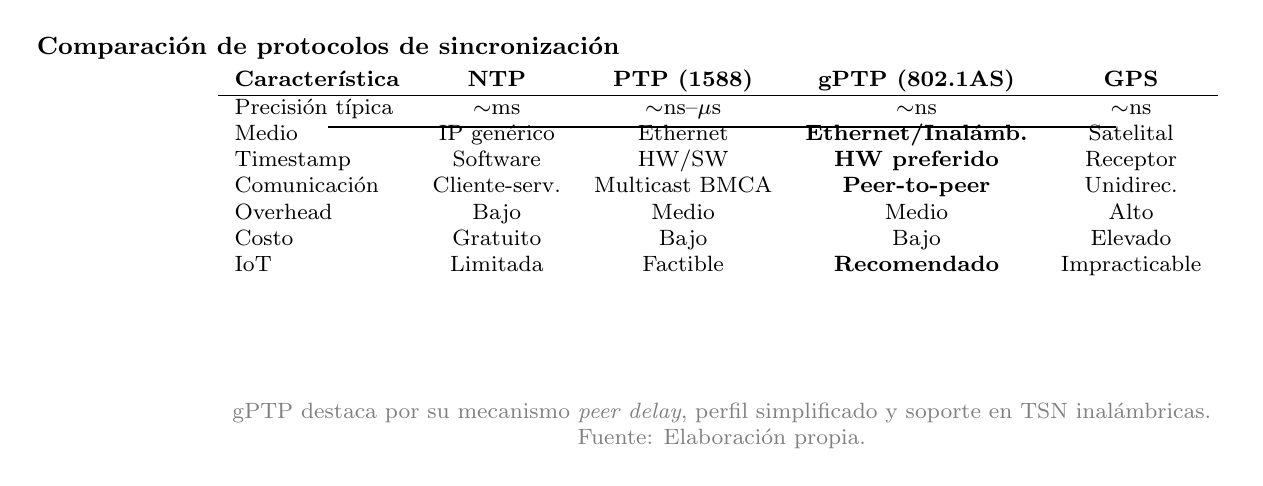
\begin{tikzpicture}
  \node[font=\small\bfseries] at (0,0.8) {Comparación de protocolos de sincronización};

  \draw[thick] (0,-0.2) -- (10,-0.2);

  \node[font=\footnotesize, align=left] at (5,-0.8) {
    \begin{tabular}{lcccc}
      \textbf{Característica} & \textbf{NTP} & \textbf{PTP (1588)} & \textbf{gPTP (802.1AS)} & \textbf{GPS} \\
      \hline
      Precisión típica & $\sim$ms & $\sim$ns--$\mu$s & $\sim$ns & $\sim$ns \\
      Medio & IP genérico & Ethernet & \textbf{Ethernet/Inalámb.} & Satelital \\
      Timestamp & Software & HW/SW & \textbf{HW preferido} & Receptor \\
      Comunicación & Cliente-serv. & Multicast BMCA & \textbf{Peer-to-peer} & Unidirec. \\
      Overhead & Bajo & Medio & Medio & Alto \\
      Costo & Gratuito & Bajo & Bajo & Elevado \\
      IoT & Limitada & Factible & \textbf{Recomendado} & Impracticable \\
    \end{tabular}
  };

  \node[font=\footnotesize, text=gray, align=center] at (5,-4) {gPTP destaca por su mecanismo \textit{peer delay}, perfil simplificado y soporte en TSN inalámbricas.\\Fuente: Elaboración propia.};
\end{tikzpicture}
\end{document}
